% Ejemplo de documento LaTeX
% Tipo de documento y tamaño de letra
\documentclass[10pt]{article}
% Preparando para documento en Español.
% Para documento en Inglés no hay que hacer esto.
\usepackage[spanish]{babel}
\selectlanguage{spanish}
\usepackage[utf8]{inputenc}
% EL titulo, autor y fecha del documento
\title{Tiro parabólico con FORTRAN y gnuplot}
\author{Rios Quijada Danira}
\date{10 de Marzo de 2015}
% Aqui comienza el cuerpo del documento
\usepackage{graphicx}
\begin{document}
% Construye el título
\maketitle
\section{Tiro parabólico con FORTRAN}
En esta práctica, primeramente realizamos un programa en FORTRAN para calcular la posición de un objeto lazado con tiro parabólico, en ciertos instantes de tiempo, el programa también calcula la y máxima y la x máxima,asi como el tiempo total en el aire; todo esto dependiendo de la velocidad inicial y del ángulo de tiro.Todos estos calculos se basan en las ecuaciones de tiro parabólico, descritas a continuación:
\space
\space
\begin{tabular}{l}
$x=v_{0}tcos(\theta)$\\
$y=v_{0}tsin(\theta)- \frac{1}{2}gt^2$
\end{tabular}
\subsection{Código}
\begin{tabular}{l}
El código que utilizamos para realizar el programa fue el siguiente:\\
\begin{verbatim}
!************************************************
!This program plots projectile motion of an object.
!The program requires user input for initial velocity
!and angle of the object.The algorithm uses a time
!step of 0.01 second i.e. it calculates object's
!location in the x and y plane every 0.01 second.
!**********By: Waleed Ishaque, 2013**************
program tiro_parabolico

implicit none

real, parameter :: g = 9.81 !Valor de la gravedad
real, parameter :: pi=4.0*ATAN(1.0)
real, parameter :: deltat = 0.01

integer, parameter :: npts= 2000 

real, dimension (1:npts) :: x,y,t
real :: xi, yi, vi, radianes, theta
real :: xmax, ymax, tiempo 

integer :: i

write (*,*), 'Deme las coordenadas iniciales de x en m'
read *, xi
write (*,*), 'Deme las coordenadas iniciales de y en m'
read *, yi
write (*,*), 'Deme la velocidad inicial del proyectil en m/s'
read *, vi
write (*,*), 'Deme el angulo inicial de tiro en grados'
read *, theta

radianes = (theta*pi)/180.0


xmax = xi+((vi*vi*sin(2*radianes))/(g))
ymax = yi+(((vi*vi)*(sin(radianes)*sin(radianes)))/(2*g))
tiempo = (2*vi*sin(radianes))/(g)

!Registramos los datos calculados
open (1, file="tiro.dat")

!Calculando la posicion para cada t(i)
do i=1, npts
t(i)=float(i)*deltat
x(i) = xi + (vi*cos(radianes)*t(i))
y(i) = yi + (vi*sin(radianes)*t(i)) - ((0.5*g)*t(i)*t(i))

!Registrando resultados
write (1,*) x(i), y(i)
if (y(i)<0) exit
end do

print *, "#####################################################"
print *, "Un tiro parabolico con:"
print *, "coordenadas iniciales x=",xi,"y=",yi
print *, "velocidad inicial", vi,"m/s"
print *, "y un angulo de", theta, "grados"
print *, "durara en el aire un tiempo de:", tiempo,"s"
print *, "alcanzara una h maxima de:", ymax,"m"
print *, "tendra un alcanze maximo en el eje x de:", xmax,"m"

CLOSE (1)
end program tiro_parabolico
\end{verbatim} \\
\end{tabular}
\newpage
\subsection{Resultados}
Cabe denotar que en el código se cambia la salida estándar de los datos de posición a un archivo, llamado ``tiro.dat'', el cual utilizaremos posteriormente para graficar con gnuplot.una vez concluido el programa, lo compilamos, he aquí los resultados al ejecutarlo con los ángulos de 90,0, 60 y 30 grados.
\subsubsection{90 grados}
\begin{center}
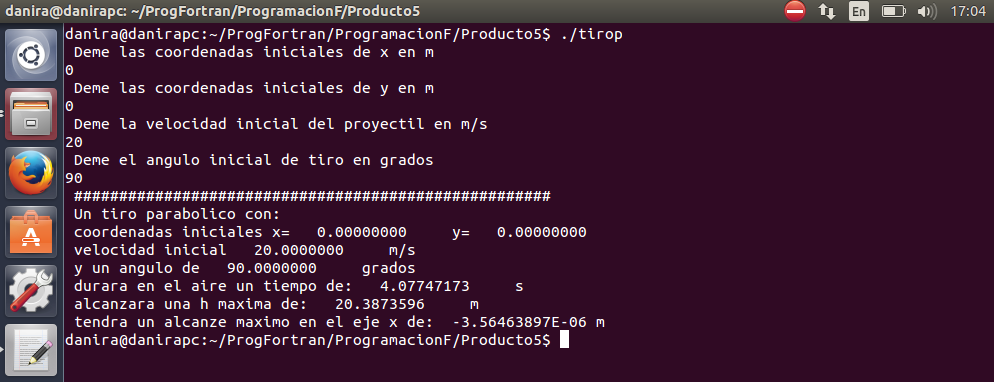
\includegraphics[scale=0.5]{90grados.PNG}
\end{center}
\subsubsection{0 grados}
\begin{center}
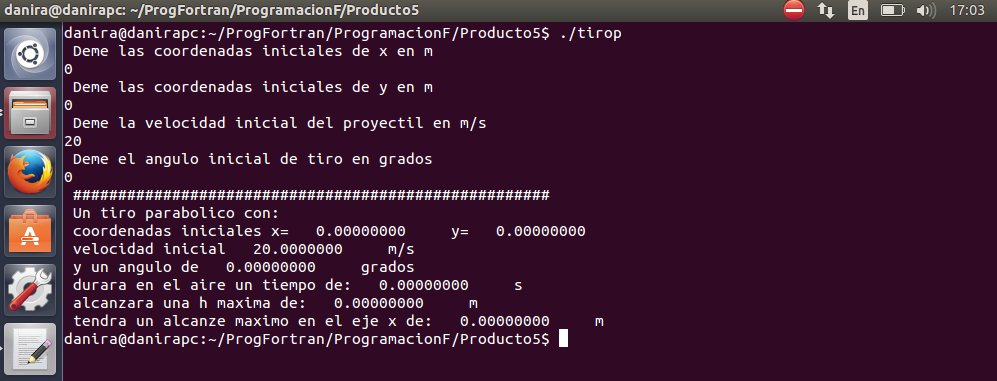
\includegraphics[scale=0.5]{0grados.PNG}
\end{center}
\subsubsection{60 grados}
\begin{center}
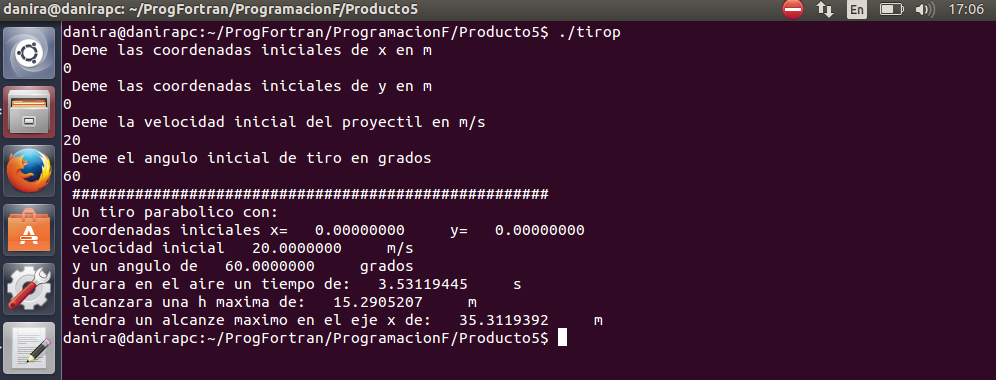
\includegraphics[scale=0.5]{60grados.PNG}
\end{center}
\subsubsection{30 grados}
\begin{center}
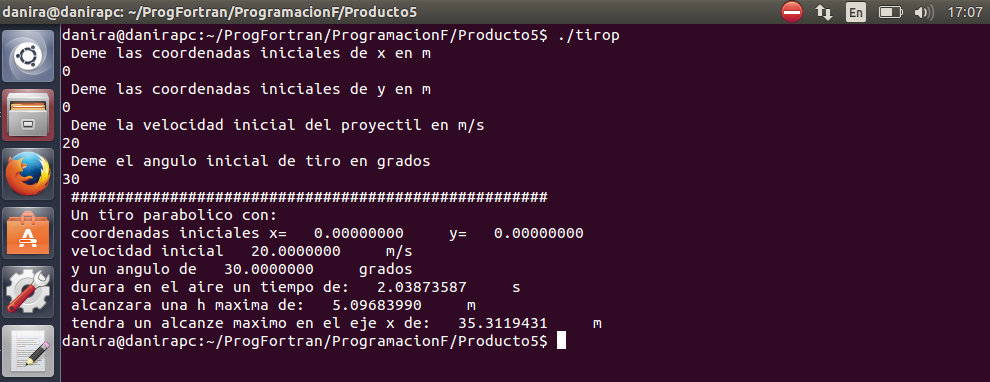
\includegraphics[scale=0.5]{30grados.PNG}
\end{center}
\newpage
\section{Graficando con Gnuplot}
En esta parte de la práctica nos enfocamos en graficar la información que nos arrojó el archivo ``tiro.dat'', para eso utilizamos gnuplot y el siguiente código.
\begin{tabular}{l}
\begin{verbatim}
gnuplot>set term png
gnuplot>set output 'tirogrados.png'
gnupltot>plot 'tiro.dat'
\end{verbatim}\\
Obteniendo el siguiente resultado para cada ángulo de prueba;
\end{tabular}
\subsection{90 grados}
\begin{center}
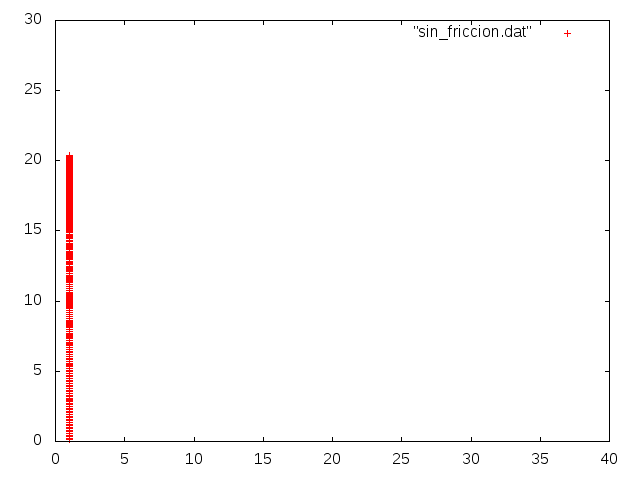
\includegraphics[scale=0.5]{90.png}
\end{center}
\subsection{0 grados}
\begin{center}
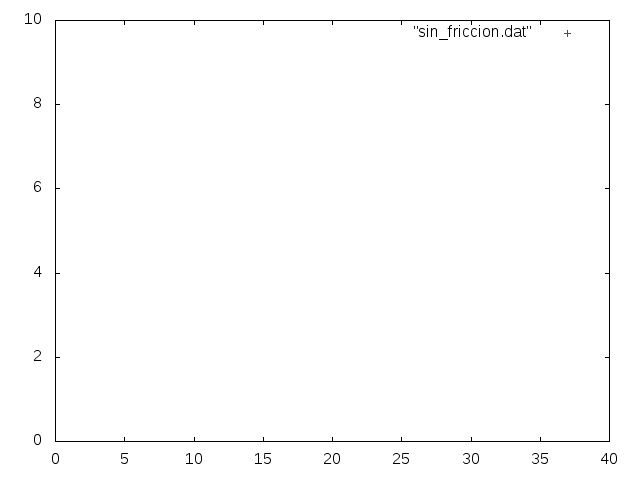
\includegraphics[scale=0.5]{0.png}
\end{center}
\subsection{60 grados}
\begin{center}
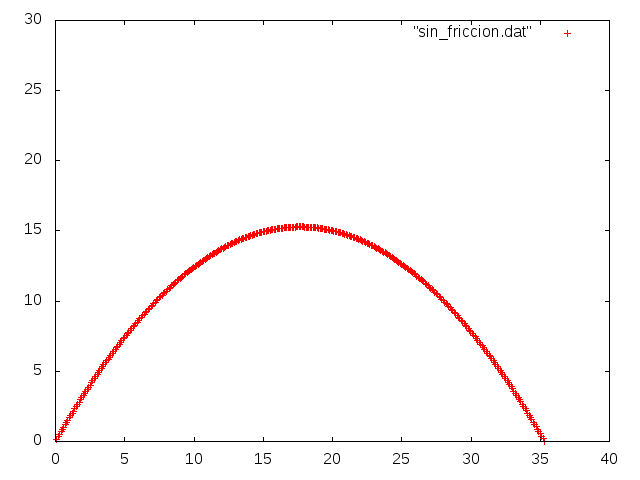
\includegraphics[scale=0.5]{60.png}
\end{center}
\subsection{30 grados}
\begin{center}
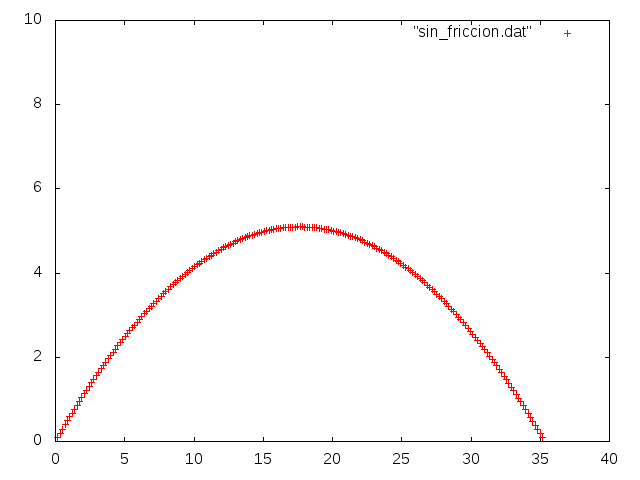
\includegraphics[scale=0.5]{30.png}
\end{center}


% Nunca debe faltar esta última linea.
\end{document}
